\chapter{Teorie zavedení operačního systému}
Pro celou analýzu a následnou stavbu infrastruktury, o~které práce uvažuje, je důležité teoretické pochopení jednotlivých kroků probíhajících od zapnutí serveru až po zavedení operačního systému. Tato kapitola se věnuje popsání jednotlivých standardů a protokolů využívaných při zavádění obrazů disků.


\section{Bare metal server}

S~přesunem IT infrasktruktury do \uv{cloudu} se v~našem průmyslu začínají objevovat nové výrazy, mezi které patří i bare metal. Nejjednodušeji řečeno, bare metal server je klasický dedikovaný server s~novým, pěkným jménem.

Ukáži na příkladu: pokud si zákazník objedná bare metal server, přístup k~hardwaru má pouze on a s~nikým ho nesdílí. Šířka pásma na síťové kartě tedy patří jen jemu a může ji celou využít.


\section{Provisioning a frameworky pro tento účel}

Pokud v~IT oblasti potkáme výraz \uv{provisioning}, obyčejně tím myslíme sérii kroků, během kterých připravíme server s~předurčeným operačním systémem, daty a dalším vybraným softwarem. Následně na serveru připravíme připojení k~síti. Mezi typické kroky patří:

\begin{itemize}
\item vybrání serveru z~databáze volných strojů,
\item nainstalování odpovídajícího softwaru (operační systém, ovladače pro hardware, aplikace),
\item konfigurace nainstalovaného softwaru z~předchozího kroku (nastavení připojení k~síti, tj. přiřazení IP adresy, brány, atp.).
\end{itemize}

Po provedení kroků se systém restartuje a načte nový operační systém. Server je zde již připraven k~použití.

Pro provisioning existuje řada nástrojů (frameworků), které se tuto činnost snaží zautomatizovat. Nástroje se většinou ve své funkčnosti překrývají, můžeme je tedy poměrně dobře porovnat. Porovnání se bude věnovat další kapitola.

\section{Zavedení kódu s~PXE}

PXE (Pre eXecution Environment) je metodou zavedení nějakého kódu (klasicky zavaděče) na koncovém zařízení pouze pomocí jeho síťové karty. PXE je definován na základě standardů internetových protokolů a služeb široce využívaných v~průmyslovém světě. Jmenovitě to jsou TCP/IP, DHCP, TFTP, které standardizují formu komunikace mezi serverem a klienty\cite{bootp-rfc} \cite{tftp-rfc}. Metoda byla prvně popsána v~roce 1999 \cite{pxe-spec}.

PXE standard pracuje v~následující krocích:

\begin{figure}[h]\centering
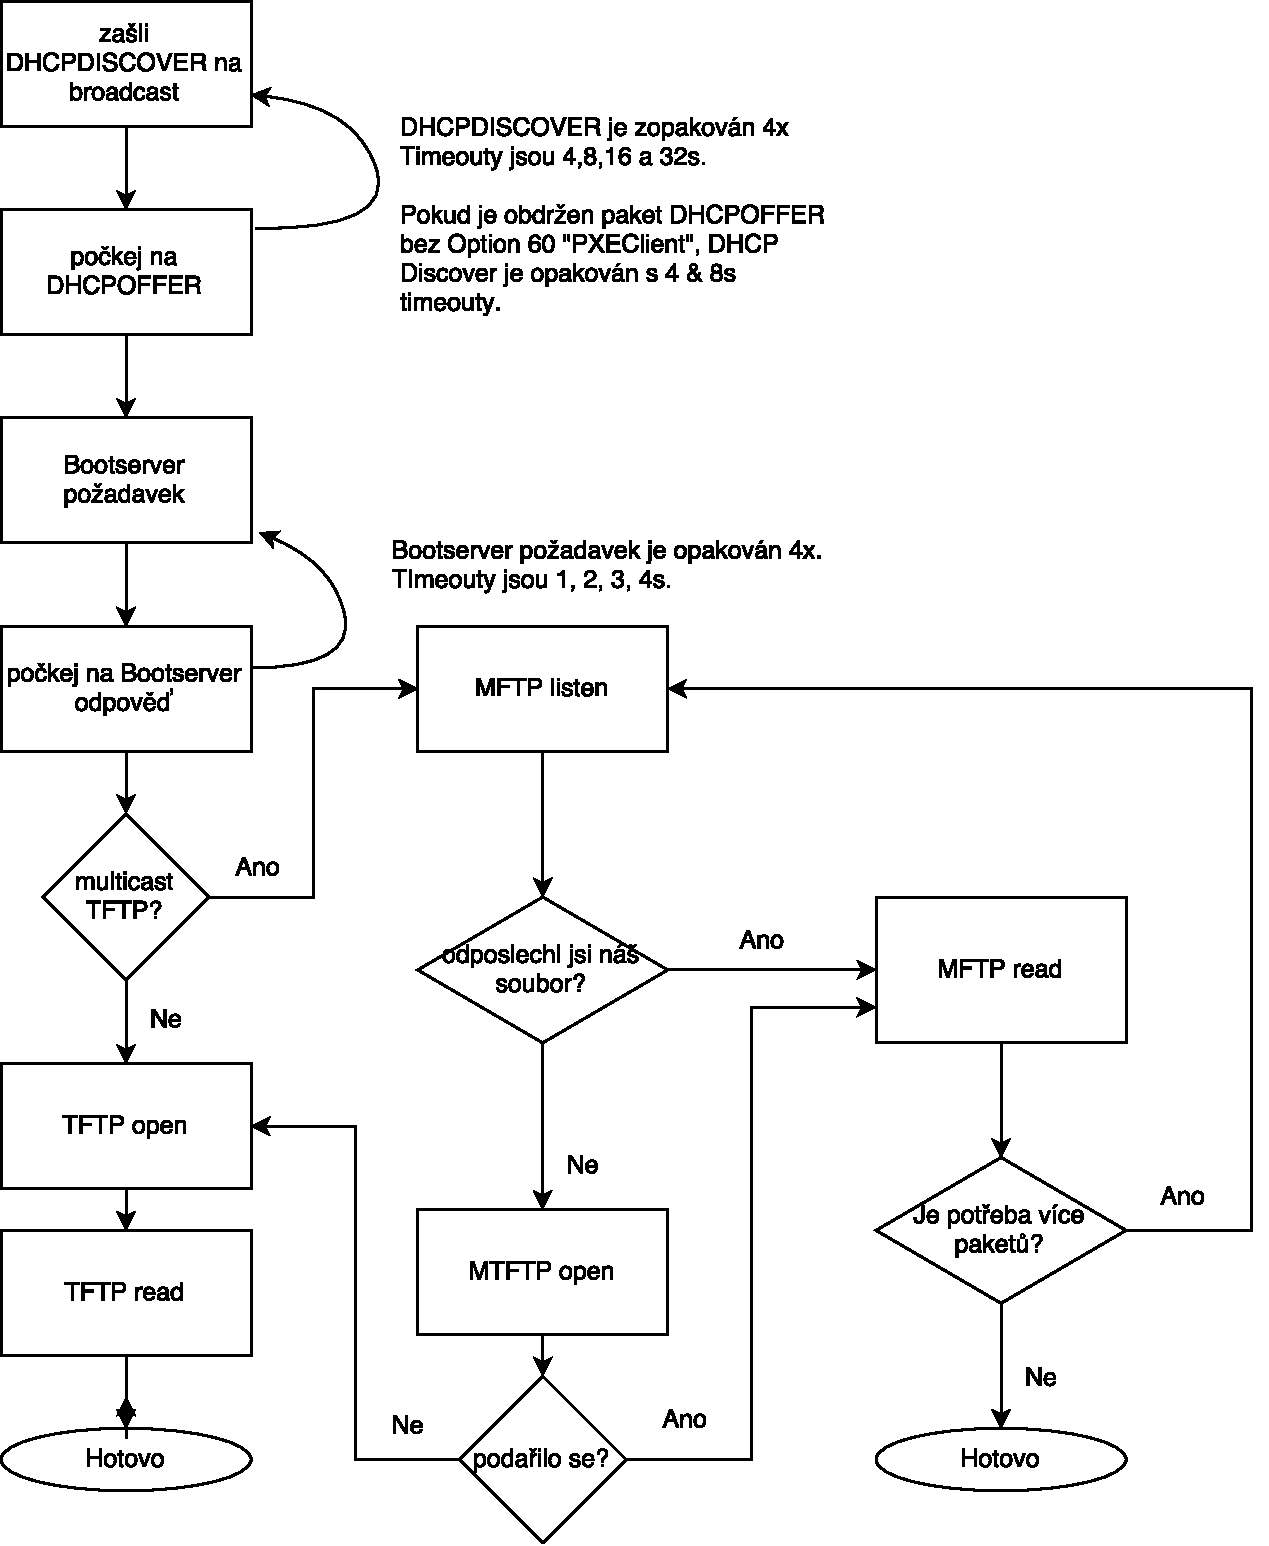
\includegraphics[width=1\textwidth]{files/pxe-flow.pdf}
	\caption{Diagram popisující průběh dle PXE}\label{fig:float}
\end{figure}

\begin{enumerate}

\item  Klient zahájí komunikaci zasláním DHCPDISCOVER paketu na broadcast adresu. K~tomu se využije standartního portu DHCP - 67 na UDP. Tento paket obsahuje rozšíření, podle kterého server pozná, že paket příchází od klienta s~implementovaným PXE protokolem. Konkrétně tedy DHCP Option 60, nastavena na PXEClient:Arch:xxxxx:UNDI:yyyzzz. (Předpokládáme, že DHCP server toto rozšíření podporuje.)

\item  Odpoví na standardním DHCP reply portu (UDP 68) paketem DHCPOFFER. Každá zpráva obsahuje klasické DHCP parametry - IP adresu klienta a další možnosti nastavené administrátorem serveru.

\item Z~DHCPOFFER paketu si klient zaznamená:
\begin{itemize}
\item IP adresu klienta,
\item seznam Boot serverů z~PXE tagu,
\item Discovery Control Options,
\item IP adresu Multicast Discovery.

\end{itemize}

\item  Pokud si klient vybere IP adresu nabídnutou DHCP službou, pak musí dokončit standartní DHCP průběh zasláním požadavku na adresu (paketu DHCPREQUEST) a poté počkáním na potvrzení požadavku od služby -- obdržením paketu DHCPACK.

\item  klient si vybere a objeví Boot server. Tento objevovací paket může být zaslán na broadcast (port 67), multicast (port 4011) nebo na unicast (port 4011). Toto záleží na nastavení obdržené v~předchozím přijatém DHCPOFFER paketu obsahující rozšiřující PXE tagy. Paket je stejný jako počáteční DHCPDISCOVER v~kroku 1, jen je organizován jako DHCPREQUEST a obsahuje:

\begin{itemize}
\item IP adresu přiřazenou klientovi z~DHCP,
\item tag pro identifikátor klienta (UUID),
\item tag pro klientovo UNDI,
\item tag pro klientovu achitekturu serveru,
\item DHCP Option 60 - nastavenou na PXEClient:Arch:xxxxx:UNDI:yyyzzz.
\end{itemize}

\item  Boot server vyšle na unicast klientovi paket DHCPACK na klientův zdrojový port. Tento paket obsahuje:

\begin{itemize}
\item jméno zaváděcího souboru
\item konfigurační parametry MTFTP \footnote{Multicast Trivial File Transfer Protocol}
\end{itemize}

\item  Klient stáhne spustitelný soubor buď pomocí standardního TFTP (port 69), nebo MTFTP (potom přiřazený port nalezneme v~Bootserver ACK paketu). Kam se server uloží, záleží na architektuře procesoru klienta.
\item  Klient rozhodne, zda je potřebný test staženého souboru. Pokud je test zapotřebí, klient zašle další DHCPREQUEST boot serveru požadující identifikační údaje staženého souboru. Tyto identifikační údaje stáhne a provede test, zda je soubor správný.

\item  Konečně, pokud podmínka kroku 8 proběhla pozitivně, PXE klient začne vykonávat kód právě staženého souboru.
\end{enumerate}

\section{Zavaděč operačního systému}

Pomocí výše uvedené série kroků do počítače chceme nahrát určitý kód. Tím kódem je zavaděč systému -- pro naše využití bylo využito bootloaderu pxelinux (patřící do kolekce zavaděčů syslinux). Zavaděčem nazýváme krátký kód, uložený v~tabulce MBR \footnote{Master Boot Record}, nebo boot sektoru jednoho z~oddílů disku. Účelem zavaděče je, aby do operační paměti počítače nakopíroval další, větší program -- tím je např. jádro operačního systému. Následně přeskočí na zkopírovaný kód a tím mu předá řízení počítače.


Zavaděče lze rozdělit do dvou kategoríí \cite{syslinux-abc}:
\begin{enumerate}

\item na primární (first-stage) -- jsou přímo obsaženy na hardware počítače. Na IBM-kompatibilních PC se tento zavaděč nazývá BIOS,
\item a sekundární (second-stage), které jsou zavolány primárním zavaděčem. Mezi ně patří právě syslinux, nebo dobře známý GRUB \cite{grub}.
\end{enumerate}

\subsection{Syslinux (pxelinux)}

V~porovnání s~GRUB je syslinux velmi jednoduchým zavaděčem \cite{syslinux-grub-comparsion}. Ve skutečnosti syslinux je kolekcí zavaděčů, každý zavaděč pro jiný účel:

\begin{enumerate}

\item syslinux je určen  pro bootování ze souborového systému FAT,
\item isolinux, pro bootování z~ISO 9660 filesystému, který je používán na CD,
\item pxelinux je určen pro bootování ze síťového serveru (tedy naše řešení),
\item extlinux -- bootování ze souborového systému ext2/ext3.
\end{enumerate}

\section{Automatizace instalace linuxových distribucí}

Následující sekce popisuje způsoby instalace linuxových distribucí bez interakce člověka. Bohužel tento proces pro všechny distribuce nebyl unifikován. Je tedy nutné použít více instalátorů v~jednom prostředí. Příští strany se budou věnovat instalátorům pro operační systémy Debian (instalátor pod názvem Preseed) a Red Hat Enterprise Linux (Kickstart).
%\subsection{Instalační skripty}

%Na různých linuxových distribucích můžeme balíčkové manažery kombinovat. Bohužel prvotní instalace - a také nástroj, pomocí kterého tento proces vykonáváme, je specifický ke každé distribuci . Pokud tedy budeme chtít provozovat heterogenní prostředí, s velikou pravděpodobností se nevyhneme použití několika instalátorů vedle sebe. Následující podkapitoly

\subsubsection{Automatizace instalace OS Debian pomocí Preseed}

\label{preseed}

Při instalaci operačního systému Debian a distribucí na něm založených, preseeding (pozn. v~překladu do češtiny přednastavení) nám umožňuje odpovědět na otázky při instalaci OS, které bychom jinak byli nuceni vyplnit ručně. Díky tomu můžeme plně automatizovat většinu instalací. Preseeding dokonce obsahuje nějaké funkce, které přes manuální instalaci nejsou dostupné. Celá tato konfigurace je obsah skriptu předložený instalaci. Následující odstavce ukazují, jak skript může být předložen a co by měl obsahovat.

\paragraph{Způsoby preseedingu}

Existují tři metody, jak skript instalaci předložit. Těmi jsou: initrd, soubor a předložení po síti.

\begin{itemize}
\item \mintinline{latex}{initrd} --  preseed konfiguraci předáme instalaci už v~ram disku; načtení skriptu se provede hned na začátku instalace. Můžeme přeskočit všechny otázky. Podmínkou je soubor \mintinline{latex}{preseed.cfg} uložený v~kořeni initrd.
\item \mintinline{latex}{soubor} -- v~tomto případě je konfigurace uložena na bootovacím médiu (tj. CD nebo USB flash disk). Načtení skriptu se provede hned po připojení média, tj. hned po dotazech na direktivy (otázky) o~jazyku instalace a rozvržení klávesnice.
\item \mintinline{latex}{ze sítě} --  načtení preseed skriptu proběhne hned po automatické konfiguraci síťových rozhraní. Boot parametr obsahující řetězec, odkud je soubor stažen, se nazývá \mintinline{latex}{preseed/url=http://server/preseed.cfg}.
\end{itemize}


V~případě této bakalářské práce je využito třetí možnosti, tj. stažení konfiguračního souboru pomocí HTTP protokolu. I~když načítání preseed konfigurace z~initrd se zdá jako nejzajímavější způsob, generování initrd instalátoru je poměrně komplexní proces.


\paragraph{Preseed soubor}

Preseed soubor je plain text soubor, ve kterém každý řádek obsahuje jednu odpověď na jednu \mintinline{latex}{debconf} direktivu. Jeden řádek obsahuje čtyři pole oddělené mezerou (nebo tabulátorem). Na příkladu
\begin{minted}{bash}
d-i mirror/suite string stable
\end{minted}
\begin{itemize}

\item \mintinline{latex}{d-i} -- první pole je tzv. vlastník direktivy; \uv{\mintinline{latex}{d-i}} je značka pro direktivy spojené s~instalátorem,
\item \mintinline{latex}{mirror/suite} je identifikátor a typ otázky oddělené lomítkem,
\item \mintinline{latex}{string stable} jsou jsou datový typ a hodnota odpovědi. Pokud řádek obsahuje další mezeru, považuje se za část odpovědi.
\end{itemize}




\subsubsection{Automatizace instalace CentOS/RHEL pomocí Kickstart}

\label{kickstart}
Kickstart je způsob automatizované instalace od společnosti RedHat. Kvůli této vazbě je tedy kompatibilní s~operačnímy systémy vázanými na tuto společnost, jmenovitě Red Hat Enterprise Linux (zkráceně RHEL), CentOS, Fedora.

Základem Kickstart instalace jsou tři prvky: malý bootovací obraz disku, konfigurační soubor a repozitář s~jednotlivými balíčky. Díky PXE instalaci obraz disku a kickstart soubor nemusí být  uložen na záznamovém médiu připojeném k~serveru. Kickstart nabízí širokou škálu možností, jak si instalaci přizpůsobit vlastní potřebě. Pěkným a užitečným způsobem, jak toto nastavit je jeden plain text soubor (\mintinline{latex}{ks.cfg}).

Soubor obsahuje část s~příkazy odkazující na jednotlivé kroky při instalaci. V~souboru předáme stejné parametry, které bychom provedli, pokud bychom instalovali interaktivně.

Kickstart soubor \mintinline{latex}{ks.cfg} se skládá z~těchto částí:

\begin{itemize}

\item nastavení klávesnice a jazyka operačního systému,
\item způsob autentifikace,
\item diskové rozdělení,
\item výběr bootloaderu,
\item seznam balíčků, které se na stroj budou instalovat,
\item a konečně vlastní příkazy, které se mají provést v~okamžiku, co skončí instalace (tzv. post-install skript).
\end{itemize}

Další ze zajímavých vlastností ks.cfg je částečně automatizovaná instalace, případně aktualizace. Instalátor se poté zeptá jen na otázky, které mu nebyly podsunuty v~konfiguračním souboru (mezi toto může například patřit rozdělení disku, které můžeme chtít u~každého serveru jiné). Některé možnosti aktualizace operačního systému pokmocí kickstartu jsou ale omezené -- například není možné aktualizovat verze balíčků.


\paragraph{Rozdělení disku}

Následující část pojednává o~možnostech kickstart instalace při rozdělení disků. Příkazy níže je možné vložit do konfiguračního souboru (\mintinline{latex}{ks.cfg}).

\mintinline{latex}{autopart} -- automaticky vytvoří diskové oddíly -- 1 GB a více pro root oddíl (\mintinline{latex}{/}), swap oddíl a boot oddíl podle příslušící architektury. Tento příkaz též přijímá parametry \mintinline{latex}{--encrypted} a \mintinline{latex}{--passphrase=PASS}.

\mintinline{latex}{ignoredisk} -- zapříčiní, že disk nebude využit. Parametr poté je\\ \mintinline{latex}{--drives=disk1,disk2,...} Druhým využitím příkazu je parametr\\ \mintinline{latex}{--use-only=disk1}, pomocí kterého určíme, pouze jaké disky máme použít.

\mintinline{latex}{raid} vytvoří software RAID. Struktura příkazu vypadá takto:
\begin{minted}{bash}
raid <mntpoint> --level=<level> --device=<mddevice> <partitions*>
\end{minted}

\mintinline{latex}{Mntpoint} je místo, kde bude vytvořený raidový oddíl připojen. Podmínkou je, že oddíl připojený na \mintinline{latex}{/boot} musí být RAID typu 1 (To samé platí i pro root oddíl, pokud nemáme zvláštní boot oddíl). Parametr level nám říká typ RAIDu  (0, 1, 4, 5, 6, nebo 10).

\mintinline{latex}{part / partition} -- vytvoří diskový oddíl na disku. K~zajímavým parametrům patří \mintinline{latex}{<mntpoint>}, \mintinline{latex}{--fstype} (případně \mintinline{latex}{--noformat}), \mintinline{latex}{--size}.

\mintinline{latex}{bootloader} -- specifikuje, jak by měl být bootloader instalován. Pomocí parametru \mintinline{latex}{--location} nastavíme oddíl (případně pozici Master Boot Recordu, pokud nastavíme \mintinline{latex}{--location=mbr}), kde má být záznam zapsán. Parametr \mintinline{latex}{--driveorder} říká, který disk je první v~pořadí v~nastavení BIOSu.

		\mintinline{latex}{clearpart} odstraní všechny diskové oddíly na discích specifikovaných v~parametru \mintinline{latex}{--drives}. S~pomocí \mintinline{latex}{--initlabel} vytvoříme label standardní k~naší architektuře, tedy GPT, či MBR.


\subsubsection{Disková rozvržení}

Před úspěšnému dokončení instalace operačního systému na server si musíme zodpovědět několik otázek. Před kopírováním systémových souborů musí být cílové médium (většinou hard disk) nastaveno. Nastavením je myšlena série kroků, do které patří

\begin{itemize}

\item partitioning, neboli vytvoření oddílů -- jednotlivé oddíly disků jsou části disku (ať už fyzického nebo logického), se kterými můžeme libovolně nezávisle manipulovat. Diskový oddíl obsahuje svůj vlastní souborový systém, připadně pododdíly,
\item naformátování disku, při kterém na oddíl zavedeme souborový systém,
\item vytvoření zavaděče disku,
\item nakopírování souborů na disk.
\end{itemize}


\section{Formáty diskových oddílů}


Na počítačích s~procesorem z~rodiny x86 (IBM PC kompatibilní) je proces bootování obyčejně řešen jedním ze dvou způsobů. Tím prvním a zároveň starším je BIOS-MBR, nebo novější UEFI-GPT. Následující odstavce přiblíží, jak metody fungují.

% Metoda UEFI-GPT je modernější, a proto podporuje užití většího počtu diskový oddílů, kdy jednotlivé oddíly můžou mít i větší velikost. V porovnaní s BIOS-MBR zvyšuje též rychlost a bezpečnost bootování.

\subsection{Standardní proces bootování s~MBR}

% http://www.pcguide.com/ref/mbsys/bios/bootSequence-c.html

MBR je starým standardem pro rozdělování oddílů disku a stále je ve velké míře používán. MBR (master boot record), se nachází na úplném začátku disku a obsahuje metadata o~tom, jak jsou na zařízení logické oddíly organizovány. Master Boot Record též obsahuje spustitelný kód, který je schopen prohledávat oddíly a najít na nich operační systém. A~následně spustit spustitelný kód/proceduru operačního systému.


Na MBR disku je možné mít pouze 4 oddíly. Pro vytvoření více oddílů je potřeba nastavit tu čtvrtou jako \uv{rozšířenou}  (tj. \uv{extended}), ve které je možné vytvořit pod-oddíly (též logické disky). Tím, že MBR využívá 32 bitů na adresu oddílu, je maximální velikost jednoho do 2TB. Takto nějak vypadá typické rozdělení MBR:
\newpage



\begin{figure}[H]\centering
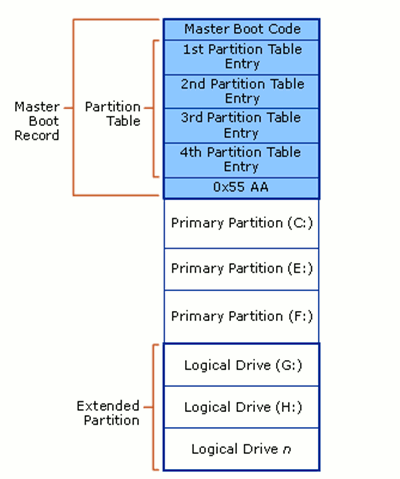
\includegraphics[width=0.5\textwidth]{files/mbr-disk-layout.png}
	\caption{MBR rozvržení disku \cite{gpt-mbr-pic}}\label{fig:float}
\end{figure}



Jak vidíme na obrázku výše, MBR má několik nevýhod. Vedle již zmíněné maximální velikosti oddílu 2TB a maximálně 4 logických oddílů, to je též fakt, že MBR je jediné místo, kde se nachází informace o~diskovém rozdělení. Pokud se tedy někdy poruší, celý disk se stane nečitelným.


% Standartní bootovací proces BIOS-MBR od zapnutí počítače po načtení operačního systému na počítačích IBM-PC kompatibilních se skládá z následujících kroků:
% \begin{itemize}
%
% \item Zapnutí počítače -- Po zapnutí či reštartu serveru sa procesoru pošle signál RESET,
%  který na sběrnicích ukončí všechny aktivity a nastaví obsah vybraných registrů na počáteční hodnoty. Procesor se potom spustí v 16b reálném módu.
% \item Spuštění BIOS kódu -- Po spuštění počítače procesor vždy nastaví obsah instrukčního ukazatele (ip – instruction pointer) na výrobcem zvolenou adresu reset vektoru
% (například pro procesor 80836 to je fyzická adresa 0xfffffff0) a začne vykonávat instrukce na nadcházejících adresách. Reset vektor ukazuje do oblasti, která obsahuje kód BIOSu. BIOS představuje firmware počítače a implementuje základní program poskytující služby na komunikaci s hardware. Jeho programový kód je uložený v ROM, EEPROM nebo flash paměti umístěné na základní desce počítače. Mezi základní úlohy BIOSu při bootovaní patří testování (POST) a inicializace hardware. Následně BIOS vyvolá přerušení int 19h.
% Vyvolaním tohoto přerušení resp. služby se BIOS na základě svojí konfigurace pokusí najít bootovací zařízení (pevný disk, CD, DVD a pod.), které obsahuje bootovací sektor. Bootovací sektor je úplně první sektor, resp. oblast velká 512 bajtů, která se nachází na CHS adrese 0/0/1 (cylinder 0, hlava 0, sektor 1) příslušného bootovacího zařízení. Aby byl tento sektor platný, musí obsahovat tzv. boot sektor podpis. To
% znamená, že bootovací sektor musí být zakončený dvojicí bajtů 0x55,
% 0xaa.
%
% Na paměťových médiích, které je možné rozdělit na více diskových
% oddílů, se první sektor nazývá master boot record (MBR). V ostatních případech, kdy bootovací sektor se nachází na oddílu, nazývame ho volume boot record (VBR). BIOS ale mezi tím nerozlišuje. Snaží se jen najít platný bootovací sektor (sektor
% s boot podpisem), jehož obsah následně přesune na předurčenou adresu do RAM paměti a předá mu řízení.
% \item Spuštění kódu MBR/VBR -- MBR resp. VBR je přesunutí do paměti RAM na fyzickou adresu 0x7c00.
% Segmentový registr cs a registr ip se nastaví tak, aby také ukazovali
% na stejnou adresu (klasicky cs = 0x0000; ip = 0x7c00). Program
% umístěný na této adrese je následně spuštěn. Ve většině případů
% MBR obsahuje krátký program -- primární zavaděč (primary bootloader),
% jehož úlohou je nalezení aktivního oddílu a následně předání
% řízení do VBR tohto oddílu. VBR většinou obsahuje kód sekundárního zavaděče, ktorý je závislý na operačním systému. Klasicky jeho
% hlavní úlohou je najít a nahrát do paměti RAM a spustit obsah sektorů,
% na kterých je umístěný soubor skutečného zavaděče operačního
% systému.
% \end{itemize}


\subsection{Standardní proces bootování s~GPT}

GPT je posledním standardem pro rozdělování oddílů na disku, současně je částí UEFI standardu. Využívá globálně unikátních identifikátorů (GUID), pomocí kterých definuje oddíl. Pro systém založený na UEFI tedy je nezbytné, aby využíval GPT. Je teoreticky možné vytvořit neomezený počet oddílů -- na většině operačních systémů je ale toto číslo omezeno na 128. Narozdíl od MBR, které je omezeno na 2TB, jeden oddíl může být velký až $ 2^{64} $ bloků (64 bit adresa). Při bloku velkém 512 bajtů je to 9.44 ZB (1 ZB je miliarda TB). Na diagramu \ref{gpt-pic} vidíme rozvržení disku s~GPT.
\newpage

\begin{figure}[h]\centering
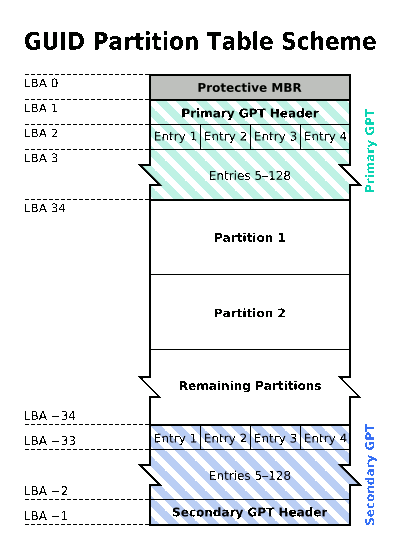
\includegraphics[width=0.5\textwidth]{files/gpt-partition-scheme.png}
	\caption{GPT rozvržení disku \cite{gpt-mbr-pic}}\label{gpt-pic}
\end{figure}

Jak ukazuje obrázek \ref{gpt-pic}, primární GPT se nachází na začátku disku a sekundární na konci. To je jedna z~funkcionalit, co dělá GPT účinnější než MBR. GPT ukládá záložní hlavičku a tabulku oddílů na konci disku, takže pokud se nějakým způsobem primární poškodí, může být zachráněna a obnovena ze sekundární. Také obsahuje CRC32 opravné součty pro detekování chyb v~hlavičce anebo tabulce oddílů. Dále můžeme vidět \uv{Protective MBR} v~prvním sektoru disku. Pomocí tohoto hybridního nastavení můžeme počítač s~biosem zavést z~disku s~GPT rozdělením, se zavaděčem uloženým v~části \uv{Protective MBR}. Tato funkcionalita je též ochranou před poškozením od nástrojů, které o~GPT neví.
